\newif\ifshowsolutions
\showsolutionstrue
\documentclass{article}
\usepackage{listings}
\usepackage{amsmath}
\usepackage{subfig}
\usepackage{amsthm}
\usepackage{amsmath}
\usepackage{amssymb}
\usepackage{graphicx}
\usepackage{mdwlist}
\usepackage{geometry}
\usepackage{titlesec}
\usepackage{palatino}
\usepackage{mathrsfs}
\usepackage{fancyhdr}
\usepackage{paralist}
\usepackage{todonotes}
\usepackage{tikz}
\usepackage{float} % Place figures where you ACTUALLY want it
\usepackage{comment} % A hack to toggle sections
\usepackage{ifthen}
\usepackage{mdframed}
\usepackage{verbatim}
\usepackage{listings}
\usepackage{bbm}
\usepackage{upquote} % Prevents backticks replacing single-quotes in verbatim
\usepackage[strings]{underscore}
\usepackage[colorlinks=true]{hyperref}
\usetikzlibrary{positioning,shapes,backgrounds}

\geometry{margin=1in}
\geometry{headheight=2in}
\geometry{top=2in}

\setlength{\marginparwidth}{2.15cm}
\setlength{\parindent}{0em}
\setlength{\parskip}{0.6\baselineskip}

\rhead{}
\lhead{}

% Spacing settings.
\titlespacing\section{0pt}{12pt plus 2pt minus 2pt}{0pt plus 2pt minus 2pt}
\titlespacing\subsection{0pt}{12pt plus 4pt minus 2pt}{0pt plus 2pt minus 2pt}
\titlespacing\subsubsection{0pt}{12pt plus 4pt minus 2pt}{0pt plus 2pt minus 2pt}
\renewcommand{\baselinestretch}{1.15}

% Shortcuts for commonly used operators.
\newcommand{\E}{\mathbb{E}}
\newcommand{\Var}{\operatorname{Var}}
\newcommand{\Cov}{\operatorname{Cov}}
\newcommand{\Bias}{\operatorname{Bias}}
\DeclareMathOperator{\argmin}{arg\,min}
\DeclareMathOperator{\argmax}{arg\,max}

% Do not number subsections and below.
\setcounter{secnumdepth}{1}

% Custom format subsection.
\titleformat*{\subsection}{\large\bfseries}

% Set up the problem environment.
\newcounter{problem}[section]
\newenvironment{problem}[1][]
  {\begingroup
    \setlength{\parskip}{0em}
    \refstepcounter{problem}\par\addvspace{1em}\textbf{Problem~\Alph{problem}\!
    \ifthenelse{\equal{#1}{}}{}{ [#1 points]}:}
  \endgroup}

% Set up the subproblem environment.
\newcounter{subproblem}[problem]
\newenvironment{subproblem}[1][]
  {\begingroup
    \setlength{\parskip}{0em}
    \refstepcounter{subproblem}\par\medskip\textbf{\roman{subproblem}.\!
    \ifthenelse{\equal{#1}{}}{}{ [#1 points]:}}
  \endgroup}

% Set up the teachers and materials commands.
\newcommand\teachers[1]
  {\begingroup
    \setlength{\parskip}{0em}
    \vspace{0.3em} \textit{\hspace*{2em} TAs responsible: #1} \par
  \endgroup}
\newcommand\materials[1]
  {\begingroup
    \setlength{\parskip}{0em}
    \textit{\hspace*{2em} Relevant materials: #1} \par \vspace{1em}
  \endgroup}

% Set up the hint environment.
\newenvironment{hint}[1][]
  {\begin{em}\textbf{Hint: }}
  {\end{em}}


% Set up the solution environment.
\ifshowsolutions
  \newenvironment{solution}[1][]
    {\par\medskip \begin{mdframed}\textbf{Solution~\Alph{problem}#1:} \begin{em}}
    {\end{em}\medskip\end{mdframed}\medskip}
  \newenvironment{subsolution}[1][]
    {\par\medskip \begin{mdframed}\textbf{Solution~\Alph{problem}#1.\roman{subproblem}:} \begin{em}}
    {\end{em}\medskip\end{mdframed}\medskip}
\else
  \excludecomment{solution}
  \excludecomment{subsolution}
\fi
\chead{
  {\vbox{
      \vspace{2mm}
      \large
      Machine Learning \& Data Mining \hfill
      Caltech CS/CNS/EE 155 \hfill \\[1pt]
      Set 2\hfill
      January $13^\text{th}$, 2023 \\
    }
  }
}

\begin{document}
\pagestyle{fancy}



%%%%%%%%%%%%%%%%%%%%%%%%%%%%%%
% POLICIES
%%%%%%%%%%%%%%%%%%%%%%%%%%%%%%

\section*{Policies}
\begin{itemize}
	\item Due 9 PM PST, January $20^\text{th}$ on Gradescope. 
	\item You are free to collaborate on all of the problems, subject to the collaboration policy stated in the syllabus.
	\item In this course, we will be using Google Colab for code submissions. You will need a Google account.
\end{itemize}

\section*{Submission Instructions}
\begin{itemize}
	\item Submit your report as a single .pdf file to Gradescope (entry code K3RPGE), under "Set 2 Report". 
	\item In the report, \textbf{include any images generated by your code} along with your answers to the questions.
	\item Submit your code by \textbf{sharing a link in your report} to your Google Colab notebook for each problem (see naming instructions below). Make sure to set sharing permissions to at least "Anyone with the link can view". \textbf{Links that can not be run by TAs will not be counted as turned in.} Check your links in an incognito window before submitting to be sure. 
	\item For instructions specifically pertaining to the Gradescope submission process, see \url{https://www.gradescope.com/get_started#student-submission}.
\end{itemize}

\section*{Google Colab Instructions}
For each notebook, you need to save a copy to your drive.
\begin{enumerate}
	\item Open the github preview of the notebook, and click the icon to open the colab preview.
	\item On the colab preview, go to File $\rightarrow$ Save a copy in Drive.
	\item Edit your file name to “lastname_firstname_set_problem”, e.g.”yue_yisong_set2_prob1.ipynb”
\end{enumerate}


%%%%%%%%%%%%%%%%%%%%%%%%%%%%%%
% PROBLEM 1
%%%%%%%%%%%%%%%%%%%%%%%%%%%%%%

\newpage
\section{Comparing Different Loss Functions [30 Points]}
\materials{lecture 3 \& 4}

We've discussed three loss functions for linear classification models so far:
\begin{itemize}
\item Squared loss: $L_\text{squared} = (1 - y\mathbf{w}^T\mathbf{x})^2$
\item Hinge loss: $L_\text{hinge} = \max(0, 1 - y\mathbf{w}^T\mathbf{x})$
\item Log loss: $L_\text{log} = \ln(1 + e^{-y\mathbf{w}^T\mathbf{x}})$
\end{itemize}
where $\mathbf{w} \in \mathbb{R}^n$ is a vector of the model parameters, $y \in \{-1,1\}$ is the class label for datapoint $\mathbf{x} \in \mathbb{R}^n$, and we're including a bias term in $\mathbf{x}$ and $\mathbf{w}$.  The model classifies points according to $\text{sign}(\mathbf{w}^T\mathbf{x})$.

Performing gradient descent on any of these loss functions will train a model to classify more points correctly, but the choice of loss function has a significant impact on the model that is learned.

\problem[3]
Squared loss is often a terrible choice of loss function to train on for classification problems.  Why?

\begin{solution}

\end{solution}

\problem[9]
A dataset is included with your problem set: problem1data1.txt. The first two columns represent $x_1, x_2$, and the last column represents the label, $y \in \{-1,+1\}$.

On this dataset, train both a logistic regression model and a ridge regression model to classify the points.  (In other words, on each dataset, train one linear classifier using $L_\text{log}$ as the loss, and another linear classifier using $L_\text{squared}$ as the loss.) For this problem, you should use the logistic regression and ridge regression implementations provided within scikit-learn 
(\href{http://scikit-learn.org/stable/modules/generated/sklearn.linear_model.LogisticRegression.html}{logistic regression documentation})
(\href{http://scikit-learn.org/stable/modules/generated/sklearn.linear_model.Ridge.html}{Ridge regression documentation})
instead of your own implementations. Use the default parameters for these classifiers except for setting the regularization parameters so that very little regularization is applied.

For each loss function/model, plot the data points as a scatter plot and overlay them with the decision boundary defined by the weights of the trained linear classifier.  Include both plots in your submission. The template notebook for this problem contains a helper function for producing plots given a trained classifier.

What differences do you see in the decision boundaries learned using the different loss functions? Provide a qualitative explanation for this behavior.

\begin{solution}

\end{solution}

\problem[9]
Leaving squared loss behind, let's focus on log loss and hinge loss. Consider the set of points $S = \{(\frac{1}{2}, 3), (2, -2), (-3, 1)\}$ in 2D space, shown below, with labels $(1, 1, -1)$ respectively.

Given a linear model with weights $w_0 = 0, w_1 = 1, w_2 = 0$ (where $w_0$ corresponds to the bias term), derive the gradients $\nabla_{w}L_{\text{hinge}}$ and $\nabla_{w}L_{\text{log}}$ of the hinge loss and log loss, and calculate their values for each point in S.

\begin{center}
  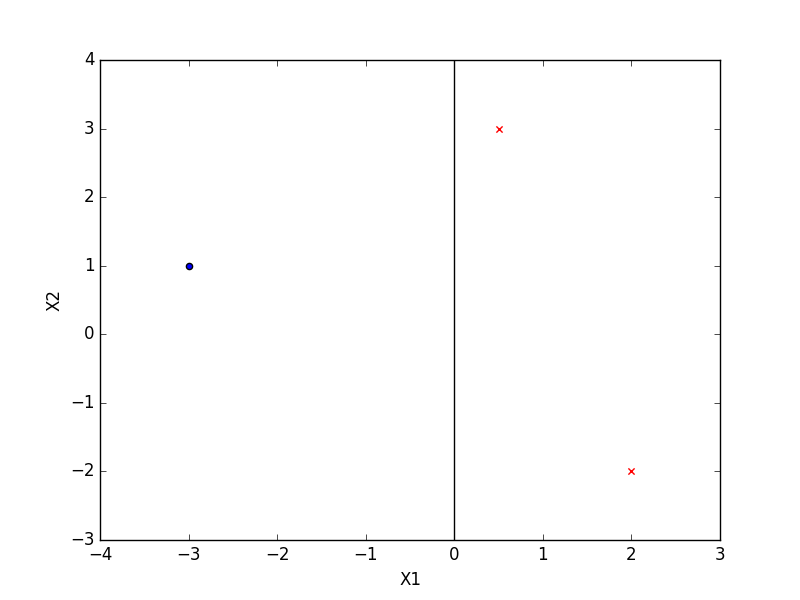
\includegraphics[width=.8\textwidth]{./plots/SimpleDatasetWithDecisionBoundary.png}
\end{center}
\begin{small}
  The example dataset and decision boundary described above. Positive instances are
  represented by red x's, while negative instances appear as blue dots.
\end{small}

\begin{solution}

\end{solution}

\problem[4]
Compare the gradients resulting from log loss to those resulting from hinge loss. When (if ever) will these gradients converge to 0? For a linearly separable dataset, is there any way to reduce or altogether eliminate training error without changing the decision boundary?

\begin{solution}

\end{solution}

\problem[5]
Based on your answer to the previous question, explain why for an SVM to be a ``maximum margin'' classifier, its learning objective must not be to minimize just $L_\text{hinge}$, but to minimize $L_\text{hinge} + \lambda\Vert w \Vert^2$ for some $\lambda > 0$.

(You don't need to prove that minimizing $L_\text{hinge} + \lambda\Vert w \Vert^2$ results in a maximum margin classifier; just show that the additional penalty term addresses the issues of minimizing just $L_\text{hinge}$.)

\begin{solution}

\end{solution}

\newpage
\section{Effects of Regularization [40 Points]}
\textit{Relevant materials: Lecture 3 \& 4}

For this problem, you are required to implement everything yourself and submit code (i.e. don't use scikit-learn but numpy is fine).
\indent\problem[4] 
In order to prevent over-fitting in the least-squares linear regression problem with continuous outputs (not classification problem), we add a regularization penalty term.
Can adding the penalty term decrease the training (in-sample) error?
Will adding a penalty term always decrease the out-of-sample errors?
Please justify your answers. Think about the case when there is over-fitting while training the model.

\begin{solution}
 
\end{solution}

\problem[4]
$\ell_1$ regularization is sometimes favored over $\ell_2$ regularization due to its ability to generate a sparse $w$ (more zero weights).
In fact, $\ell_0$ regularization (using $\ell_0$ norm instead of $\ell_1$ or $\ell_2$ norm) can generate an even sparser $w$, which seems favorable in high-dimensional problems.
However, it is rarely used.  Why?

\begin{solution}

\end{solution}

\subsection{Implementation of \texorpdfstring{$\ell_2$}{L2} regularization:}

We are going to experiment with regression for the Red Wine Quality Rating data set. The data set is uploaded on the course website, and you can read more about it here: \url{https://archive.ics.uci.edu/ml/datasets/Wine}. The data relates 13 different factors (last 13 columns) to wine type (the first column). Each column of data represents a different factor, and they are all continuous features. Note that the original data set has three classes, but one was removed to make this a binary classification problem.

Download the data for training and validation from the assignments data folder.
There are two training sets,
wine\_training1.txt (100 data points) and wine\_training2.txt (a proper subset of wine\_training1.txt containing only 40 data points), and one test set, wine\_validation.txt (30 data points). You will use the wine\_validation.txt dataset to evaluate your models.

We will train a \emph{$\ell_2$-regularized logistic regression} model on this data. Recall that the unregularized logistic error (a.k.a. log loss) is
\[E = -\sum_{i=1}^{N}\log(p(y_i | \mathbf{x}_i))\]

where $p(y_i = -1 | \mathbf{x}_i)$ is
\[\frac{1}{1 + e^{\mathbf{w}^T\mathbf{x}_i}}\]

and $p(y_i = 1 | \mathbf{x}_i)$ is
\[\frac{1}{1 + e^{-\mathbf{w}^T\mathbf{x}_i}},\]
where as usual we assume that all $\mathbf{x}_i$ contain a bias term.
The $\ell_2$-regularized logistic learning objective is 
\begin{align*}
  E &= -\sum_{i=1}^{N}\log(p(y_i | \mathbf{x}_i)) + \lambda\mathbf{w}^T\mathbf{w} \\
    &= -\sum_{i=1}^{N} \log \left( \frac{1}{1 + e^{-y_i\mathbf{w}^T\mathbf{x}_i}} \right) + \lambda\mathbf{w}^T\mathbf{w} \\
    &= -\sum_{i=1}^{N} \left(\log \left( \frac{1}{1 + e^{-y_i\mathbf{w}^T\mathbf{x}_i}} \right) - \frac{\lambda}{N}\mathbf{w}^T\mathbf{w}\right).
\end{align*}
Implement SGD to train a model that minimizes the $\ell_2$-regularized logistic learning, i.e. train an $\ell_2$-regularized logistic regression model.  Train the model with 15 different values of $\lambda$ starting with $\lambda_0 = 0.00001$ and increasing by a factor of 5, i.e. $$\lambda_0 = 0.00001, \lambda_1 = 0.00005, \lambda_2 = 0.00025, ..., \lambda_{14} = 61,035.15625.$$
\par

\textbf{Some important notes:} 
\begin{itemize}
    \item Terminate the SGD process after 20,000 epochs, where each epoch performs one SGD iteration for each point in the training dataset.
    \item You should shuffle the order of the points before each epoch such that you go through the points in a random order (hint: use \texttt{numpy.random.permutation}).
    \item Use a learning rate of $5 \times 10^{-4}$, and initialize your weights to small random numbers. 
    \item The \textit{$\ell_2$-regularized} logistic learning objective is what you aim to minimize during the training. However, when computing the training error and the testing error, you should compute the \textit{unregularized} logistic error. 
\end{itemize}


You may run into numerical instability issues (overflow or underflow). One way to deal with these issues is by normalizing the input data $X$. Given the column for the $j$th feature, $X_{:,j}$, you can normalize it by setting $X_{ij} = \frac{X_{ij} - \overline{X_{:,j}} }{\sigma(X_{:,j})}$ where $\sigma(X_{:,j})$ is the standard deviation of the $j$th column's entries, and $\overline{X_{:,j}}$ is the mean of the $j$th column's entries. Normalization may change the optimal choice of $\lambda$; the $\lambda$ range given above corresponds to data that has been normalized in this manner. If you treat the input data differently, simply plot enough choices of $\lambda$ to see any trends.

\problem[16]
Do the following for both training data sets (wine\_training1.txt and wine\_training2.txt) and attach your plots in the homework submission (use a log-scale on the horizontal axis):

\subproblem Plot the average training error ($E_\text{in}$) versus different $\lambda$s.

\subproblem Plot the average test error ($E_\text{out}$) versus different $\lambda$s using wine\_validation.txt as the test set.

\subproblem Plot the $\ell_2$ norm of $\mathbf{w}$ versus different $\lambda$s. \medskip

 You should end up with three plots, with two series (one for wine\_training1.txt and one for wine\_training2.txt) on each plot. Note that the $E_\text{in}$ and $E_\text{out}$ values you plot should not include the regularization penalty --- the penalty is only included when performing gradient descent.

\begin{solution}

\end{solution}

\problem[4]
Given that the data in wine\_training2.txt is a subset of the data in wine\_training1.txt, compare errors (training and test) resulting from training with wine\_training1.txt (100 data points) versus wine\_training2.txt (40 data points). Briefly explain the differences.

\begin{solution}

\end{solution}

\problem[4]
Briefly explain the qualitative behavior (i.e. over-fitting and under-fitting) of the training and test errors with different $\lambda$s while training with data in wine\_training1.txt.

\begin{solution}

\end{solution}

\problem[4]
Briefly explain the qualitative behavior of the $\ell_2$ norm of $\textbf{w}$ with different $\lambda$s while training with the data in wine\_training1.txt.

\begin{solution}
   
\end{solution}

\problem[4]
If the model were trained with wine\_training2.txt, which $\lambda$ would you choose to train your final model? Why?

\begin{solution}
  
\end{solution}

% Question 3
\newpage
\section{Lasso (\texorpdfstring{$\ell_1$}{L1}) vs. Ridge (\texorpdfstring{$\ell_2$}{L2}) Regularization [25 Points]}
\textit{Relevant materials: Lecture 3}

For this problem, you may use the scikit-learn (or other Python package) implementation of Lasso and Ridge regression --- you don't have to code it yourself.

The two most commonly-used regularized regression models are Lasso ($\ell_1$) regression and Ridge ($\ell_2$) regression.
Although both enforce ``simplicity'' in the models they learn, only Lasso regression results in sparse weight vectors.
This problem compares the effect of the two methods on the learned model parameters.

\problem[11] 
The tab-delimited file problem3data.txt on the course website contains 1000 9-dimensional datapoints.  The first 9 columns contain $x_1,\ldots,x_9$, and the last column contains the target value $y$.

\subproblem
Train a linear regression model on the problem3data.txt data with Lasso regularization for regularization strengths $\alpha$ in the vector given by \texttt{numpy.linspace(0.01, 3, 30)}.
On a single plot, plot each of the model weights $w_1, ..., w_9$ (ignore the bias/intercept) as a function of $\alpha$.

\subproblem
Repeat \textbf{i.} with Ridge regression, and this time using regularization strengths $\alpha \in \{1, 2, 3, \ldots, 1e4\}$.


\subproblem
As the regularization parameter increases, what happens to the number of model weights that are exactly zero with Lasso regression?
What happens to the number of model weights that are exactly zero with Ridge regression?

\medskip
\lstset{
  basicstyle=\small\ttfamily,
  breaklines=true,
  columns=fullflexible
}

\begin{solution}

\end{solution}

\problem[7]

\subproblem
In the case of 1-dimensional data, Lasso regression admits a closed-form solution.
Given a dataset containing $N$ datapoints, each with $d = 1$ feature, solve for
\[\underset{w}{\argmin} \Vert\mathbf{y} - \mathbf{x}w\Vert^2 + \lambda\Vert w\Vert_1,
\]
where $\mathbf{x} \in \mathbb{R}^{N}$ is the vector of datapoints and $\mathbf{y} \in \mathbb{R}^N$ is the  vector of all output values corresponding to these datapoints. Just consider the case where $d = 1$, $\lambda \geq 0$, and the weight $w$ is a scalar.

This is linear regression with Lasso regularization.

\begin{subsolution}
 
\end{subsolution}

\subproblem
In this question, we continue to consider Lasso regularization in 1-dimension. Now, suppose that $w \neq 0$ when $\lambda = 0$. Does there exist a value for $\lambda$ such that $w = 0$? If so, what is the smallest such value?

\begin{subsolution}
  
\end{subsolution}

\problem[7]
\subproblem
Given a dataset containing $N$ datapoints each with $d$ features, solve for
\[\underset{\mathbf{w}}{\argmin} \Vert\mathbf{y} - \mathbf{X}\mathbf{w}\Vert^2 + \lambda\Vert\mathbf{w}\Vert_2^2
\]
where $\mathbf{X} \in \mathbb{R}^{N \times d}$ is the matrix of datapoints and $\mathbf{y} \in \mathbb{R}^N$ is the  vector of all output values for these datapoints. Do so for arbitrary $d$ and $\lambda \geq 0$.

This is linear regression with Ridge regularization.

\begin{subsolution}
 
\end{subsolution}

\subproblem In this question, we consider Ridge regularization in 1-dimension. Suppose that $w \neq 0$ when $\lambda = 0$. Does there exist a value for $\lambda > 0$ such that $w = 0$? If so, what is the smallest such value?

\begin{subsolution}

\end{subsolution}
\newpage

\section{Convexity and Lipschitz Continuity [10 Points]}
% \textit{Relevant materials: Lecture 3}

\emph{This problem develop the notions of convexity and Lipschitz-continuity. These are widely applicable concepts in machine learning that we will explore further over the next few assignments.} \\

A set $C$ is convex if the line segment between any two points in $C$ lies in $C$, i.e.,
if for any $x_1, x_2 \in C$ and any $\theta$ with $0 \leq \theta \leq 1$, we have
\[\theta x_1  + (1 - \theta)x_2 \in C\]
% Similarly, let $\Omega$ be a convex subset of a real vector space. Then, for a function $f:\Omega\to\mathbb{R}$, and $A\subseteq \Omega$, the function is said to be convex in $A$ if and only if for any points $x_1, x_2 \in A$ and for any $\lambda\in(0,1)$, we have:
% \[f(\lambda x_1 + (1-\lambda)x_2) \leq \lambda f(x_1) + (1-\lambda)f(x_2)\]

\problem[5] Let $C \subseteq \mathbb{R}^n$ be a convex set, with $x_1, \dots, x_k\in C$, and let $\theta_, \dots, \theta_k \in \mathbb{R}$ satisfy $\theta_i\geq 0$, and 
$\theta_1 + \dots + \theta_k = 1$. Show that $\theta_1 x_1 + \dots + \theta_k x_k \in C$. \\
\emph{Hint: The definition of convexity is that this holds for $k = 2$; you must show it for arbitrary $k$.}\\

\begin{solution}
    
\end{solution}

\vspace{0.5cm}

\problem[5 Extra Credit] Consider a metric space $(X, d_X)$ and $(Y, d_Y)$, where $X$ and $Y$ are sets and $d_X$ and $d_Y$ denote the metric on $X$ and $Y$, respectively. Then, a function $f:X\to Y$ is said to be $K$-Lipschitz continuous if and only if there exists a real-valued constant $K\geq 0$ such that, for all $x_1$ and $x_2$ in $X$, we have:
\[\frac{d_Y(f(x_1), f(x_2))}{d_X(x_1, x_2)} \leq K\]
Consider the metric spaces $(D_i, \|\cdot\|)$ for all $i\in\{1, \dots, t+1\}$, where $\|\cdot\|$ is the $L_2$ norm metric. Suppose that the sequence of functions $f_1, \dots, f_t$ satisfies the property that $f_i: D_i \to D_{i+1}$ is $L$-Lipschitz continuous for all $i \in \{1, 2, \cdots, t\}$. Then, show that their composition $(f_t \circ f_{t-1} \circ \cdots \circ f_1)$ is $L^t$-Lipschitz continuous.\\

\begin{solution}
    
\end{solution}
\end{document}

%%% Local Variables:
%%% mode: latex
%%% TeX-master: t
%%% End: